\subsubsection{Annealing Hamiltonian}\label{sec:annealing-hamiltonian}

Suppose we start with a QUBO:
\begin{equation*}
    E(\mathbf{x}) = \mathbf{x} Q \mathbf{x}^T
\end{equation*}
For example:
\begin{equation*}
    E(x_1, x_2) = x_1 + x_2 - 2 x_1 x_2
\end{equation*}
This is just a classical optimization problem. Now we convert it into an Ising formulation (\autopageref{eq:ising-energy-function}):
\begin{equation*}
    H_{\text{Ising}} = \sum_i h_i s_i + \sum_{i>j} J_{ij} s_i s_j
\end{equation*}
Then we move from classical spins to quantum spins, and we get the quantum Ising Hamiltonian (\autopageref{eq:quantum-ising-hamiltonian}):
\begin{equation*}
    \hat{H}_{\text{Ising}} = \sum_i h_i Z_i + \sum_{i > j} J_{ij} Z_i Z_j
\end{equation*}
Now we have built a quantum Hamiltonian that encodes the optimization problem. We have a mathematical operator whose energies correspond to the QUBO cost. For example:
\begin{equation*}
    h_1 = 2, \quad h_2 = -1, \quad J_{12} = 3
\end{equation*}
With the Hamiltonian:
\begin{equation*}
    \hat{H}_{\text{Ising}} = 2 Z_1 - Z_2 + 3 Z_1 Z_2
\end{equation*}
To find the ground state of this Hamiltonian, we can compute the energy for each configuration of the spins. For example:
\begin{center}
    \begin{tabular}{@{} c c c @{}}
        \toprule
        $s_1$ & $s_2$ & $E(s_1, s_2)$ \\
        \midrule
        $+1$ & $+1$ & $2(1) - 1(1) + 3(1)(1) = 4$ \\
        $+1$ & $-1$ & $2(1) - 1(-1) + 3(1)(-1) = -2$ \\
        $-1$ & $+1$ & $2(-1) - 1(1) + 3(-1)(1) = -4$ \\
        $-1$ & $-1$ & $2(-1) - 1(-1) + 3(-1)(-1) = 0$ \\
        \bottomrule
    \end{tabular}
\end{center}
The ground state is the configuration with the lowest energy, which is $s_1 = -1$ and $s_2 = +1$, with energy $-4$. This means that the optimal solution to the original QUBO problem is $x_1 = 0$ and $x_2 = 1$ (since $s_i = 2 x_i - 1$).

\highspace
\textcolor{Red2}{\faIcon{exclamation-triangle} \textbf{The Problem.}} If the number of spins is small, like in the example above, we can easily compute the energy for each configuration and find the ground state. However, as the number of spins increases, the number of configurations grows exponentially ($2^n$), making it infeasible to compute the energy for all configurations. So, the question is: \textbf{\emph{instead of checking all $2^n$ configurations one by one, can a quantum system naturally evolve toward the ground state?}}.

\newpage

\begin{flushleft}
    \textcolor{Green3}{\faIcon{check-circle} \textbf{The main idea of Quantum Annealing}}
\end{flushleft}
Instead of starting directly from the problem Hamiltonian $\hat{H}_{\text{Ising}}$, we \hl{start from a very simple Hamiltonian whose ground state is easy to prepare}. Then we slowly \textbf{transform} that \textbf{simple Hamiltonian into the Hamiltonian encoding our optimization problem}. If the evolution is \emph{slow enough}, the \hl{quantum system tends to remain in its ground state throughout the process}. At the end, the ground state contains the solution of the optimization problem.

\highspace
\begin{definitionbox}[: Quantum Annealing]
    The name \emph{annealing} comes from metallurgy. Imagine a piece of metal: (1) heat it up; (2) at high temperature, atoms move freely; (3) cool it down slowly; (4) the atoms settle into a low-energy configuration. This process is called \textbf{annealing}.

    \highspace
    In quantum computing, we can \emph{mimic} processes using \textbf{quantum evolution} instead of temperature. The system starts in the ground state of the easy Hamiltonian and, if we evolve slowly enough, ends in the ground state of the problem Hamiltonian.

    \highspace
    Therefore, \definition{Quantum Annealing} is a \textbf{technique} that \textbf{finds the solution of an optimization problem} by encoding the problem into a Hamiltonian and then slowly transforming an easy quantum system into that problem Hamiltonian, hoping the system continuously follows the ground state until it reaches the optimal solution.

    \highspace
    The whole method relies on the \definition{Adiabatic Theorem}, which states that if a quantum system starts in the ground state and the Hamiltonian changes sufficiently slowly, the system remains in the instantaneous ground state.
\end{definitionbox}

\highspace
To achieve this, \textbf{quantum annealing uses a time-dependent Hamiltonian} of the form:
\begin{equation}\label{eq:annealing-hamiltonian}
    H(s) = -\frac{A(s)}{2} \left( \sum_i \hat{\sigma}_{x}^{(i)} \right) + \frac{B(s)}{2} \left( \sum_i h_i \hat{\sigma}_{z}^{(i)} + \sum_{i > j} J_{ij} \hat{\sigma}_{z}^{(i)} \hat{\sigma}_{z}^{(j)} \right)
\end{equation}
Called the \definition{Transverse-Field Ising Model (TFIM)}. At first glance this looks intimidating, but it is simply the \textbf{sum of two Hamiltonians}: the \textbf{Ising term} (the second part), which is along the $Z$ direction because contains Pauli-Z operators, and the \textbf{transverse field term} (the first part), which is along the $X$ direction because contains Pauli-X operators. The name \textbf{transverse field} comes from the fact that the first term creates a magnetic field that is perpendicular (transverse) to the direction of the Ising interactions (which are along the $Z$ axis).

\newpage

\begin{figure}[!ht]
    \centering
    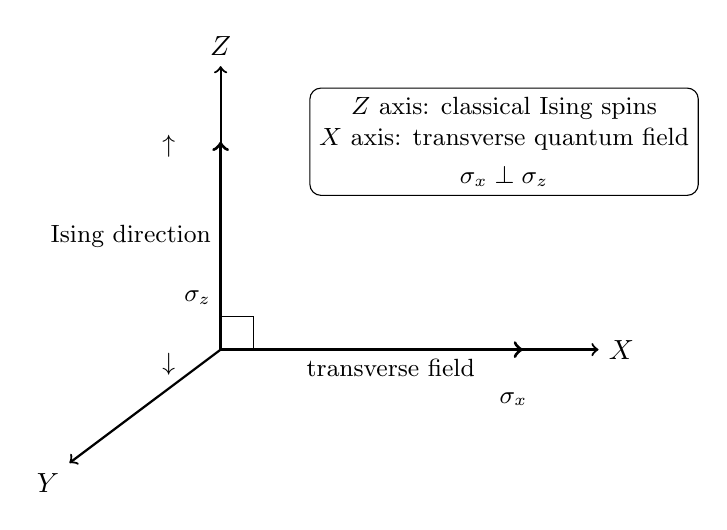
\begin{tikzpicture}[
        scale=1.2,
        axis/.style={->, thick},
        spin/.style={->, very thick},
        field/.style={->, very thick, dashed},
        lab/.style={font=\small}
    ]

        % 3D axes
        \draw[axis] (0,0) -- (4,0) node[right] {$X$};
        \draw[axis] (0,0) -- (0,3) node[above] {$Z$};
        \draw[axis] (0,0) -- (-1.6,-1.2) node[below left] {$Y$};

        % Ising spin direction along Z
        \draw[spin] (0,0) -- (0,2.2);
        \node[lab, left] at (0,1.2) {Ising direction};
        \node[lab, left] at (0,0.55) {$\sigma_z$};

        % Transverse field along X
        \draw[field] (0,0) -- (3.2,0);
        \node[lab, below] at (1.8,0) {transverse field};
        \node[lab, below] at (3.1,-0.35) {$\sigma_x$};

        % Spin examples along Z
        \node[lab] at (-0.55,2.15) {$\uparrow$};
        \node[lab] at (-0.55,-0.15) {$\downarrow$};

        % Right angle marker
        \draw (0.35,0) -- (0.35,0.35) -- (0,0.35);

        % Explanation box
        \node[draw, rounded corners, align=center, font=\small] at (3.0,2.2) {
            $Z$ axis: classical Ising spins\\
            $X$ axis: transverse quantum field\\[1mm]
            $\sigma_x \perp \sigma_z$
        };

    \end{tikzpicture}
    \caption{The quantum field acts along the $X$ direction, perpendicular to the Ising $Z$ direction.}
\end{figure}

\begin{itemize}
    \item \important{Initial Hamiltonian}:
    \begin{equation*}
        -\frac{A(s)}{2} \left( \sum_i \hat{\sigma}_{x}^{(i)} \right)
    \end{equation*}
    This first term is called \textbf{initial Hamiltonian} and its role is to create an easily-prepared quantum state.

    \textcolor{Green3}{\faIcon{question-circle} \textbf{What is $\hat{\sigma}_{x}^{(i)}$?}} $\hat{\sigma}_{x}^{(i)}$ is the Pauli-X operator acting on the $i$-th qubit. It is called the \definition{Transverse Field} and it creates quantum fluctuations (spin flips) that allow the system to explore the energy landscape.

    \textcolor{Green3}{\faIcon{check-circle} \textbf{The Standard Choice: Pauli-X Operator}} The most common choice for the initial Hamiltonian is to use the Pauli-X operator, which creates a superposition of all possible states. This is because we \textbf{want to start with a state that is not biased toward any particular solution}, \hl{allowing the system to explore the entire solution space}. Formally, the initial Hamiltonian is often chosen as:
    \begin{equation}\label{eq:initial-hamiltonian}
        H_A = -\sum_{i=1}^n X_i
    \end{equation}
    Where $X_i$ is the Pauli-X operator acting on the $i$-th qubit, and $H_A$ is the initial Hamiltonian.

    \textcolor{Green3}{\faIcon{question-circle} \textbf{Why Pauli-X operator and not Pauli-Z?}} Suppose we choose $H = -Z$. The eigenstates of $Z$ are $\ket{0}$ and $\ket{1}$, which are also the computational basis states, and the eigenvalues are:
    \begin{equation*}
        -Z\ket{0} = -1 \ket{0}, \quad -Z\ket{1} = +1 \ket{1}
    \end{equation*}
    Therefore, the ground state of $-Z$ is $\ket{0}$. But this is a \textbf{problem}, because the system is \textbf{already in the ground state} of the problem Hamiltonian (since $\ket{0}$ is also an eigenstate of $Z$). This means that the system will not evolve and we won't be able to find the solution.

    \highspace
    On the other hand, Pauli-X operator \textbf{tries to flip the spin} and creates a superposition of states. For example, choosing $H = -X$, the eigenstates of $X$ are:
    \begin{equation*}
        \ket{+} = \frac{\ket{0} + \ket{1}}{\sqrt{2}}, \quad \ket{-} = \frac{\ket{0} - \ket{1}}{\sqrt{2}}
    \end{equation*}
    With eigenvalues:
    \begin{equation*}
        -X\ket{+} = -1 \ket{+}, \quad -X\ket{-} = +1 \ket{-}
    \end{equation*}
    Therefore, the ground state of $-X$ is $\ket{+}$, which is a superposition of $\ket{0}$ and $\ket{1}$.

    \highspace
    Roughly speaking, the superposition state $\ket{+}$ does not correspond to a single candidate solution. Instead, it places the system in a quantum state that contains \textbf{all possible computational basis} states with equal amplitude. For $n$ qubits:
    \begin{equation*}
        \ket{+}^{\otimes n}
        =
        \frac{1}{\sqrt{2^n}}
        \sum_{x \in \{0,1\}^n} \ket{x}
    \end{equation*}
    Therefore, the system is not initially biased toward any particular solution. The transverse field generated by the Pauli-$X$ operators continuously induces spin flips and quantum fluctuations, \textbf{allowing the system to explore different regions of the energy landscape}. During the annealing process, these fluctuations are gradually reduced while the problem Hamiltonian is turned on, ideally guiding the system toward the ground state corresponding to the optimal solution.


    \item \important{Problem Hamiltonian}:
    \begin{equation*}
        \frac{B(s)}{2} \left( \sum_i h_i \hat{\sigma}_{z}^{(i)} + \sum_{i > j} J_{ij} \hat{\sigma}_{z}^{(i)} \hat{\sigma}_{z}^{(j)} \right)
    \end{equation*}
    This second term is called \textbf{problem Hamiltonian} and it exactly the Ising Hamiltonian we saw before (\autopageref{eq:quantum-ising-hamiltonian}). It contains the \textbf{information about the optimization problem we want to solve}. The coefficients $h_i$ and $J_{ij}$ are derived from the original QUBO problem, and they encode the cost function we want to minimize.
\end{itemize}
\textcolor{Green3}{\faIcon{question-circle} \textbf{What are $A(s)$ and $B(s)$?}} These functions \textbf{control the annealing process}. They are \textbf{time-dependent weights} that determine how much influence the initial Hamiltonian and the problem Hamiltonian have at any given time.

\highspace
Typically, at the \textbf{beginning} of the annealing process ($s=0$), we have:
\begin{equation*}
    A(0) \gg B(0)
\end{equation*}
This means that the system is dominated by the initial Hamiltonian, the Transverse Field, and the exploration of the energy landscape is strong. As \textbf{time progresses}, we gradually decrease $A(s)$ and increase $B(s)$, so that at the end of the annealing process, we have:
\begin{equation*}
    A(s) \ll B(s)
\end{equation*}
This means that the system is dominated by the problem Hamiltonian and by the optimization problem we want to solve. The hope is that if we change $A(s)$ and $B(s)$ \textbf{slowly enough}, the system will remain in its ground state throughout the evolution, and at the end, it will be in the ground state of the problem Hamiltonian, which corresponds to the optimal solution of the original QUBO problem.

\begin{figure}[!htp]
    \centering
    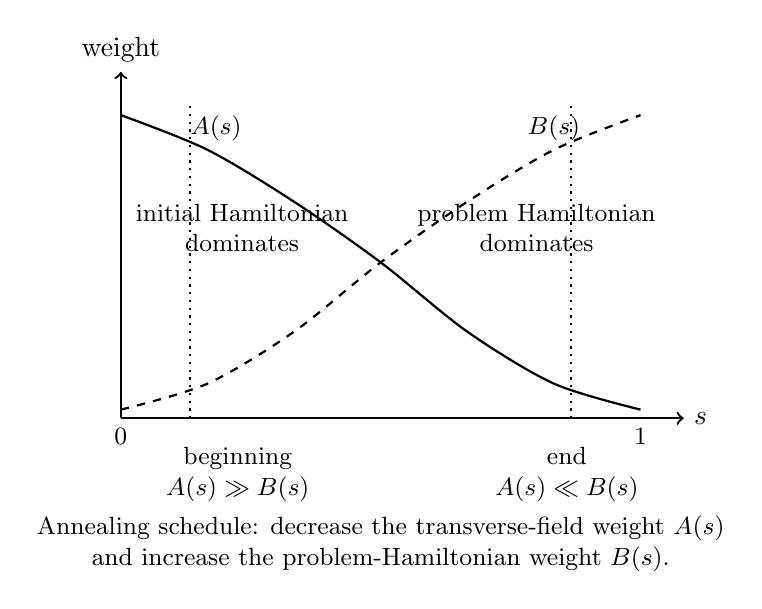
\begin{tikzpicture}[
        scale=1.1,
        axis/.style={->, thick},
        curveA/.style={thick},
        curveB/.style={thick, dashed},
        label/.style={font=\small}
    ]

        % Axes
        \draw[axis] (0,0) -- (6.5,0) node[right] {$s$};
        \draw[axis] (0,0) -- (0,4) node[above] {weight};

        % x-axis labels
        \node[label, below] at (0,0) {$0$};
        \node[label, below] at (6,0) {$1$};

        % Curves
        \draw[curveA] plot[smooth] coordinates {
            (0,3.5) (1,3.1) (2,2.5) (3,1.8) (4,1.0) (5,0.4) (6,0.1)
        };

        \draw[curveB] plot[smooth] coordinates {
            (0,0.1) (1,0.4) (2,1.0) (3,1.8) (4,2.5) (5,3.1) (6,3.5)
        };

        % Labels for curves
        \node[label] at (1.1,3.35) {$A(s)$};
        \node[label] at (5.0,3.35) {$B(s)$};

        % Beginning region
        \draw[dotted, thick] (0.8,0) -- (0.8,3.6);
        \node[label, align=center] at (1.35,-0.65) {beginning\\$A(s)\gg B(s)$};

        % End region
        \draw[dotted, thick] (5.2,0) -- (5.2,3.6);
        \node[label, align=center] at (5.15,-0.65) {end\\$A(s)\ll B(s)$};

        % Hamiltonian labels
        \node[label, align=center] at (1.4,2.2) {
            initial Hamiltonian\\
            dominates
        };

        \node[label, align=center] at (4.8,2.2) {
            problem Hamiltonian\\
            dominates
        };

        % Caption inside figure
        \node[label, align=center] at (3,-1.45) {
            Annealing schedule: decrease the transverse-field weight $A(s)$\\
            and increase the problem-Hamiltonian weight $B(s)$.
        };

    \end{tikzpicture}
    \caption{Typical annealing schedule controlled by the functions $A(s)$ and $B(s)$.}
\end{figure}